\chapter{Backend}\label{ch:backend}

Così come è stato fatto per il front end, andremo a spiegare in questa sezione gli strumenti utilizzati per gestire la parte back end del progetto. Il backend, più nel dettaglio, si occupa di gestire i dati provenienti dall'interfaccia in modo da poterli processare attraverso modelli e funzioni lato server in modo da poter tornare all'utente un risultato dei dati inviati.

Qui di seguito sono esposte le tecnologie utilizzati per far fronte alla gestione del backend.

\section{Reti Neurali e applicazioni}

Anche se nello sviluppo dell'applicativo le reti neurali sono state solo integrate è necessario definire una piccola finestra in questa tesi per fornire una contestualizzazione delle stesse in questa trattazione.

\subsection{Reti Neurali}

Una rete neurale artificiale è un sistema computazionale che sfrutta i meccanismi dell'apprendimento automatico per apprendere e abituarsi a pattern regolari cercando di emulare così il lavoro compiuto dal nostro cervello e cercando di reagire a diversi stimoli e sfide come quest'ultimo fa da ormai migliaia di anni. Il nome infatti ricalca le nozioni biologiche conosciute andando a sostituire a neuroni e dendriti che fanno da padrone nel sistema nervoso, quelli che sono dei neuroni artificiali e processi connessi che generalemente permettono al modello di essere adattivo, in modo tale che cambi la propria struttura come se fosse una funzione del tempo e dei dati che sono già stati processati.

Facendo un parallelismo biologico, il neurone biologico soggetto ad uno stimolo in ingresso proveniente da altre connessioni sinaptiche  si attiva e se il potenziale di attivazione supera una soglia definita come potenziale di azione, genera un segnale che si propaga attraverso il suo assone ad altri neuroni. Allo stesso modo, anche se spiegato in maniera semplicistica,  una rete neurale artificiale è composta da vari strati di neuroni, dove ognuno di essi è connesso a tutti i neuroni dello strato successivo e la cui connessione rappresenta quella che è l'attivazione, corrispondente in informatica ad un peso.

L'attivazione comporterà il calcolo di una Funzione di Attivazione che avrà il compito di passare il valore dei vari pesi processati allo strato seguente.Tutto questo processo continua fino a che non si arriva allo strato finale costituito dai neuroni di output che vanno a restituire il valore finale.

L'apprendimento della rete si imposta proprio alla regolazione di questi pesi fino a che l'output corrispondente all'input inviato non è quello desiderato.

\subsection{Reti Neurali utilizzate}

La tipologia di rete neurale che usano i nostri modelli è la MANN, o Memory Augmented Neural Network. Questa versione permette di usufruire di un supporto di memoria persistente che viene riservata nel momento del training e che poi viene acceduta quando si ha necessità di fare inferenza. In questo modo l'accesso ai dati è più rapido ed inoltre si limitano i dati ridondanti.

In particolare noi abbiamo utilizzato delle reti neurali per categorizzare una coppia di indumenti, o outfit, in un preciso stile e/o evento sociale, in modo da consigliare all'utilizzatore un preciso abbinamento in base alle sue richieste.

L'applicativo di basa su due principali reti neurali:
\begin{itemize}
	
\item Fashion2Events: allo stesso modo questa rete neurale restituisce un preciso evento sociale a partire da un outfit, ovvero una coppia di indumenti. Il modello è allenato a partire dal dataset USED, che contiene circa 525,000 immagini appartenenti a 14 tipi diversi di evento, divise in:
\begin{itemize}
	\item Train set: 361,000 files 
	\item Test set: 164,000 files.
\end{itemize}

Addestrandosi su questo dataset la rete riesce a comprendere qual è approssimativamente lo stile che generalmente viene usato ad un preciso evento. Nello specifico le label associate agli eventi sono: concert, graduation, meeting, mountain-trip, picnic, sea-holiday, ski-holiday, wedding, conference, exhibition, fashion, protest, sport, theater-dance.
A partire da queste label quindi ne va ad attribuire una all'outfit che ci premuriamo di salvare insieme agli altri metadati dell'outfit stesso.
	
\item Style Based Outfit Recommendation: si occupa di definire, data una coppia di indumenti, un preciso stile di abbigliamento derivante dal colore e dalle forme degli abiti. Questa rete è addestrata a partire dal dataset IQON3000  che contiene 308,347 outfits creati da 33569 utenti per mezzo di 672,335 accessori di moda.
Come anticipato prima lo stile dell'outfit si basa principalmente sul tono di un abito, che può essere più freddo o più caldo, e dalla sua silhouette, più leggiadra o meno. In particolare le categorie nelle quali il categorizzatore include gli outfits sono riportate nella figura~\ref{figura:stili}.


\end{itemize}

\begin{figure}[tbp]
	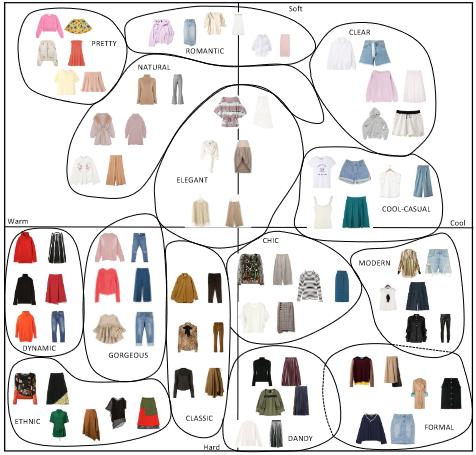
\includegraphics{img/styles}
	\caption{Label per la raccomandazione in Style Based Outfit Recommendation} \label{figura:stili} 
\end{figure}

\subsection{Segmentatore}

Per quanto riguarda la presentazione delle immagini degli indumenti è stato necessario l'uso di un segmentatore. Questo perchè altrimenti le foto sarebbero state salvate così come erano, introducendo non pochi problemi come:
\begin{itemize}
\item Estetica: lasciare nell'immagine ulteriori oggetti esterni fuori del contesto dell'indumento sarebbe stato in prima parte poco gradevole dal punto di vista visivo. 
\item Usabilità: l'eliminazione di soggetti estranei rende più intuibile che l'immagine riportata rappresenta totalmente un indumento, impedendo in questo modo incomprensioni da parte dell'utente.
\item Correttezza: la presenza di corpi estranei avrebbe potuto influenzare negativamente l'azione dei modelli che forniscono gli abbinamenti. Ad esempio, il colore dei non indumenti avrebbe potuto influire sul colore totale dell'immagine, andando così a porre in background il vero colore di interesse, ovvero quello del vestito.
\end{itemize}

In particolare, la segmentazione di un'immagine nell'elaborazione digitale delle immagini è il processo di partizione di un'immagine in regioni significative. Viene utilizzata per ottenere una rappresentazione più compatta, per estrarre degli oggetti o come strumento per l'analisi delle immagini e permette di partizionare le immagini digitali in insiemi di pixel. Lo scopo della segmentazione è semplificare e/o cambiare la rappresentazione delle immagini in qualcosa che è più significativo e facile da analizzare.

La segmentazione è di solito utilizzata per localizzare oggetti e bordi (linee, curve, ecc.). Più precisamente, la segmentazione è il processo con il quale si classificano i pixel dell'immagine che hanno caratteristiche comuni, pertanto ciascun pixel in una regione è simile agli altri della stessa regione per una qualche proprietà o caratteristica (colore, intensità o texture). Regioni adiacenti sono significativamente differenti rispetto ad almeno una di queste caratteristiche. Il risultato di un'immagine segmentata è un insieme di segmenti che, collettivamente, coprono l'intera immagine. Nel nostro caso la segmentazione è stata utilizzata al fine di trovare i bordi dell'indumento, soggetto principale della foto, e successivamente ritagliarlo dallo sfondo.

In particolare abbiamo utilizzato Detectron2 un software proprietario di FaceBook AI Research,che implementa algoritmi di object-detection che hanno ormai raggiunto lo stato dell'arte. Ai fini del progetto è stata utilizzata la funzione di object-detection per identificare il vestito (che dovrebbe ricoprire la parte preponderante della foto) e i metodi per la instance segmentation in modo da ottenere la precisa squadratura dell'oggetto stesso.

Dal punto di vista prestazionale, il risultato, dopo aver fornito l'immagine di input, viene restituito mediamente dopo pochi secondi dal modello già addestrato. Sebbene le tempistiche potrebbero sembrare larghe, in realtà per il task prefissato rispecchiano le medie temporali di altri segmentatori in commercio. Per ovviare comunque al problema di dover far attendere l'utente sul risultato in uscita dalla rete è stato provveduto un sistema di caricamento che fornisce un feedback visivo sullo stato di avanzamento dell'operazione.

A livello tecnico, l'immagine acquisita dalle API che gestiscono la fotocamera viene codificata in base64 per essere inviata al server, dove viene processata dal segmentatore che prima la riconverte in png, la elabora, per poi ritornarla al front end al fine di essere memorizzata in locale, ovviamente in caso di azione di salvataggio.

\section{Base64}

Per quanto riguarda la memorizzazione in locale e il recupero delle immagini, abbiamo avuto la necessità di doverci affidare a un sistema di codifica facile e veloce, in modo da garantire sempre elevate prestazioni e una reattività tale da consentire agli utenti prontezza d'uso dell'applicativo. Abbiamo deciso di fare affidamento in questo caso al protocollo di codifica Base64, che ha rispettato tutte le richieste implementative e prestazionali del nostro progetto.

Andando nello specifico, Base64 è un gruppo di schemi di codifica da binario a testo che rappresentano dati binari (più specificamente, una sequenza di byte a 8 bit) in un formato stringa ASCII traducendo i dati in una rappresentazione radix -64. Ogni cifra Base64 non finale rappresenta esattamente 6 bit di dati. Tre byte a 8 bit (cioè un totale di 24 bit) possono quindi essere rappresentati da quattro cifre Base64 a 6 bit.

Comune a tutti gli schemi di codifica da binario a testo, Base64 è progettato per trasportare dati archiviati in formati binari attraverso canali che supportano in modo affidabile solo contenuto di testo. Base64 è particolarmente diffuso nel Web, dove i suoi usi includono la possibilità di incorporare file di immagine o altre risorse binarie all'interno di risorse testuali come file HTML e CSS , come nel caso del nostro progetto.

\section{HTTP}

In questa trattazione non possiamo non parlare del protocollo di comunicazione e trasferimento che ci ha permesso di far interagire il front end ed il back end dell'applicativo sviluppato. Questo perchè, al fine di inviare le immagini al server per essere processate dal segmentatore o dalle reti neurali oppure per riportarle elaborate nel backend, avevamo bisogno di un protocollo facile, veloce e sicuro che stabilisse una connessione comunicativa tra i due endpoint.

Nel dettaglio HTTP, o HyperText Transfer Protocol è un protocollo del livello applicativo che, come anticipato sopra, riesce a trasmettere informazioni sia sul web che in applicazioni, con la tipica architettura client-server. Le richieste al server HTTP vengono effettuate sulla porta 80 per mezzo del protocollo TCP, o Transmission Control Protocol, a livello di trasporto.

HTTP è  un protocollo che funziona con un'architettura di tipo client-server: il client effettua una richiesta  e il server la risposta inviata da un altro host.  Nell'uso corrente,  il client corrisponde al browser e il server alla macchina su cui risiede il sito  Esistono  quindi due tipi di messaggi HTTP: messaggi di richiesta e messaggi di risposta. 

In particolare ai fini del progetto abbiamo fatto uso delle richieste POST al fine di inviare il file in base64 al server per l'elaborazione logica, mentre una richiesta GET è stata sfruttata per riprendere i dati una volta finito il processo.

\section{JSON}

JSON è un formato perfetto per lo scambio di dati fra applicazioni client/server. In particolare nel nostro progetto è stato sfruttato per codificare le informazioni da memorizzare in locale e che rappresentano gli indumenti con la relativa foto e metadati necessari affinchè questa sia processata. 
I metodi JSON che abbiamo adoperato si integrano perfettamente con il metodo di codifica delle foto catturate dall'app, ovvero in base64, fornendo addirittura un campo specifico per questo tipo di dati.

\section{Flask}

Per quanto riguarda la gestione del back end, la scelta che abbiamo fatto è stata quella di affideraci a flask. Avevamo infatti bisogno di un framework completo in python che ci permettesse di ricevere richieste dal front end in modo da gestire le chiamate agli script in Python delle reti neurali che abbiamo utilizzato.

nel dettaglio Flask è quello che possiamo definire micro-framework, dato che non ha un nucleo complesso ma può essere esteso tramite numerosi plugin ed estensioni, che espone la possibilità di mantenere un server ed un debugger, fondamentali per poter far interagire l'utente della web app con il codice delle reti neurali.

Abbiamo sfruttato la sua funzionalità di server in modo da poter ricevere ed inviare dati al front end tramite delle chiamate a richieste HTTP. I dati ricevuti, chiaramente, vengono dati in input ai vari modelli per la categorizzazione e la segmentazione che li processano e li restituiscono come output da reinviare al client.


